\documentclass[10pt,a4paper]{article}
\usepackage[margin=0.52in]{geometry}
\usepackage{graphicx}
\usepackage{booktabs}
\usepackage{float}
\usepackage{enumitem}
\usepackage{url}
\usepackage[hidelinks]{hyperref}
\setlist{nosep,leftmargin=*,topsep=2pt}
\urlstyle{same}
\setlength{\parskip}{0.2em}

\title{\textbf{Task 3: Attention Visualization \& Token Attribution}}
\author{TinyLlama Instruction Tuning Project}
\date{\today}

\begin{document}
\maketitle
\vspace{-1em}

\section*{Task description}
This analytical phase, "Attention Visualization \& Token Attribution," investigates how Low-Rank Adaptation (LoRA) mathematically shifts the internal attention mechanisms of TinyLlama. We loaded a fine-tuned LoRA checkpoint (rank 16, train on 10k Alpaca examples) and evaluated the structural routing of all 704 attention heads (32 heads $\times$ 22 layers) across 20 distinct instructional prompts. The task encapsulates multiple sub-objectives: extracting deep attention maps, implementing cosine-similarity based feature clustering to uncover semantic head groupings, mapping token attribution flows using attention rollout matrices, and generating interpretable HTML heatmaps. By empirically classifying heads as "instruction-following" or "completion-centric", we isolate and quantify the exact architectural alterations triggered by fine-tuning.

\section*{Procedure \& technical implementation}
\begin{enumerate}
  \item \textbf{Attention Map Extraction:} We isolated the base \texttt{TinyLlama-1.1B-Chat-v1.0} model and merged it with the Alpaca LoRA adapter. We monkey-patched the transformer \texttt{self\_attn.\_\_call\_\_} logic specifically over a forced sequence forward-pass to capture the raw softmax matrices $(H, L, L)$ per layer simultaneously across the 20 Alpaca inference samples.
  \item \textbf{Token Attribution (Rollout):} We simulated token influence flows from embedded input queries to generated output text. This was achieved by determining the cumulative product $R^{(l)} = \mathrm{norm}(A^{(l)}+I)\cdot R^{(l-1)}$ incrementally down the model's 22 nested layer blocks.
  \item \textbf{Clustering Analysis:} To group head behavior, we constructed a 40-dimensional feature profile for each head by concatenating mean instruction and mean completion attention scores spanning the 20 test inputs. We mapped groups utilizing average-linkage hierarchical clustering over spatial cosine distances with $k=3$ distinct clusters.
  \item \textbf{Head Function Classification:} We established an algorithmic classification threshold per head. If the mean attention mass directed toward prompt tokens exceeded the local-window response attention, the head was tagged as \textbf{instruction-following}. Conversely, if attention leaned toward recent generation context, it was tagged as \textbf{completion}.
  \item \textbf{Visualization Exports:} Comprehensive comparative heatmaps scaling the base vs LoRA distributions were assembled. The pipeline outputted 20 distinct topological HTML attention graphs alongside Python clustering artifacts natively stored within \path{results/task3/}.
\end{enumerate}

\section*{Metrics Calculation Methodology}
To ensure reproducibility, performance shifts within internal weights were tracked via the following metrics:
\begin{itemize}
  \item \textbf{Instruction-Following vs. Completion classification:} A binary toggle determined per-head. Calculated mathematically by taking the average attention weight addressing the "prompt" token indices and subtracting the average weight traversing the latest "completion" token sequence window.
  \item \textbf{Attention Focus:} A measurement of graph sharpness per evaluated sequence. Calculated by extracting the maximum attention weight scalar applied to any single target token by a head.
  \item \textbf{Attention Entropy:} Derived utilizing standard Shannon information theory over the softmax probability vectors mapping token correlation. A lower entropy figure inherently signifies a highly concentrated and deterministic focal target.
  \item \textbf{$\Delta$Net (Layer Level):} Measured comprehensively across layer clusters by subtracting the net instruction-completion orientation of the target baseline model from the identical structure within the LoRA modification.
\end{itemize}

\section*{Results}
{\small
\begin{table}[H]
\centering
\caption{Head classification and attention statistics (20 Alpaca prompts, 704 heads). Source: \texttt{analysis\_summary.json}.}
\label{tab:t3}
\footnotesize
\begin{tabular}{@{}lcccc@{}}
\toprule
\textbf{Model} & \textbf{Instruction-following} & \textbf{Completion} & \textbf{Attn.\ focus} & \textbf{Entropy} \\
\midrule
Base  & 445 (63.2\%) & 259 (36.8\%) & 0.5445 & 0.7355 \\
LoRA  & 417 (59.2\%) & 287 (40.8\%) & 0.5999 & 0.7289 \\
$\Delta$ & $-28$ heads ($-4.0\%$) & $+28$ & $+10.2\%$ & $-0.9\%$ \\
\bottomrule
\end{tabular}
\end{table}

\textbf{Key findings.}
\begin{itemize}
  \item \textbf{28 heads} (4\%) shifted instruction$\to$completion after LoRA; all 22 layer $\Delta$net values are negative, confirming a uniform completion-mode amplification across depth.
  \item \textbf{Attention focus +10.2\%} (0.5445$\to$0.5999) with slightly lower entropy: LoRA sharpens prompt-token attribution without dispersing attention.
  \item \textbf{Most affected layers:} 16 ($\Delta{=}{-}0.00301$), 12 ($-0.00248$), 13 ($-0.00243$), 9 ($-0.00236$), 2 ($-0.00208$) --- mid-to-late layers dominate LoRA's recalibration.
  \item \textbf{Stable instruction heads:} L8H11, L15H16, L11H8, L15H20 retain near-identical scores in both models; L1H30 and L14H30 completion heads are amplified in magnitude by LoRA.
  \item \textbf{Cluster structure preserved:} 3-group dendrogram topology identical in base and LoRA; LoRA makes within-cluster refinements only.
\end{itemize}
}

\section*{Evidence (screenshots)}
\begin{figure}[H]
\vspace{0.3cm}
\centering
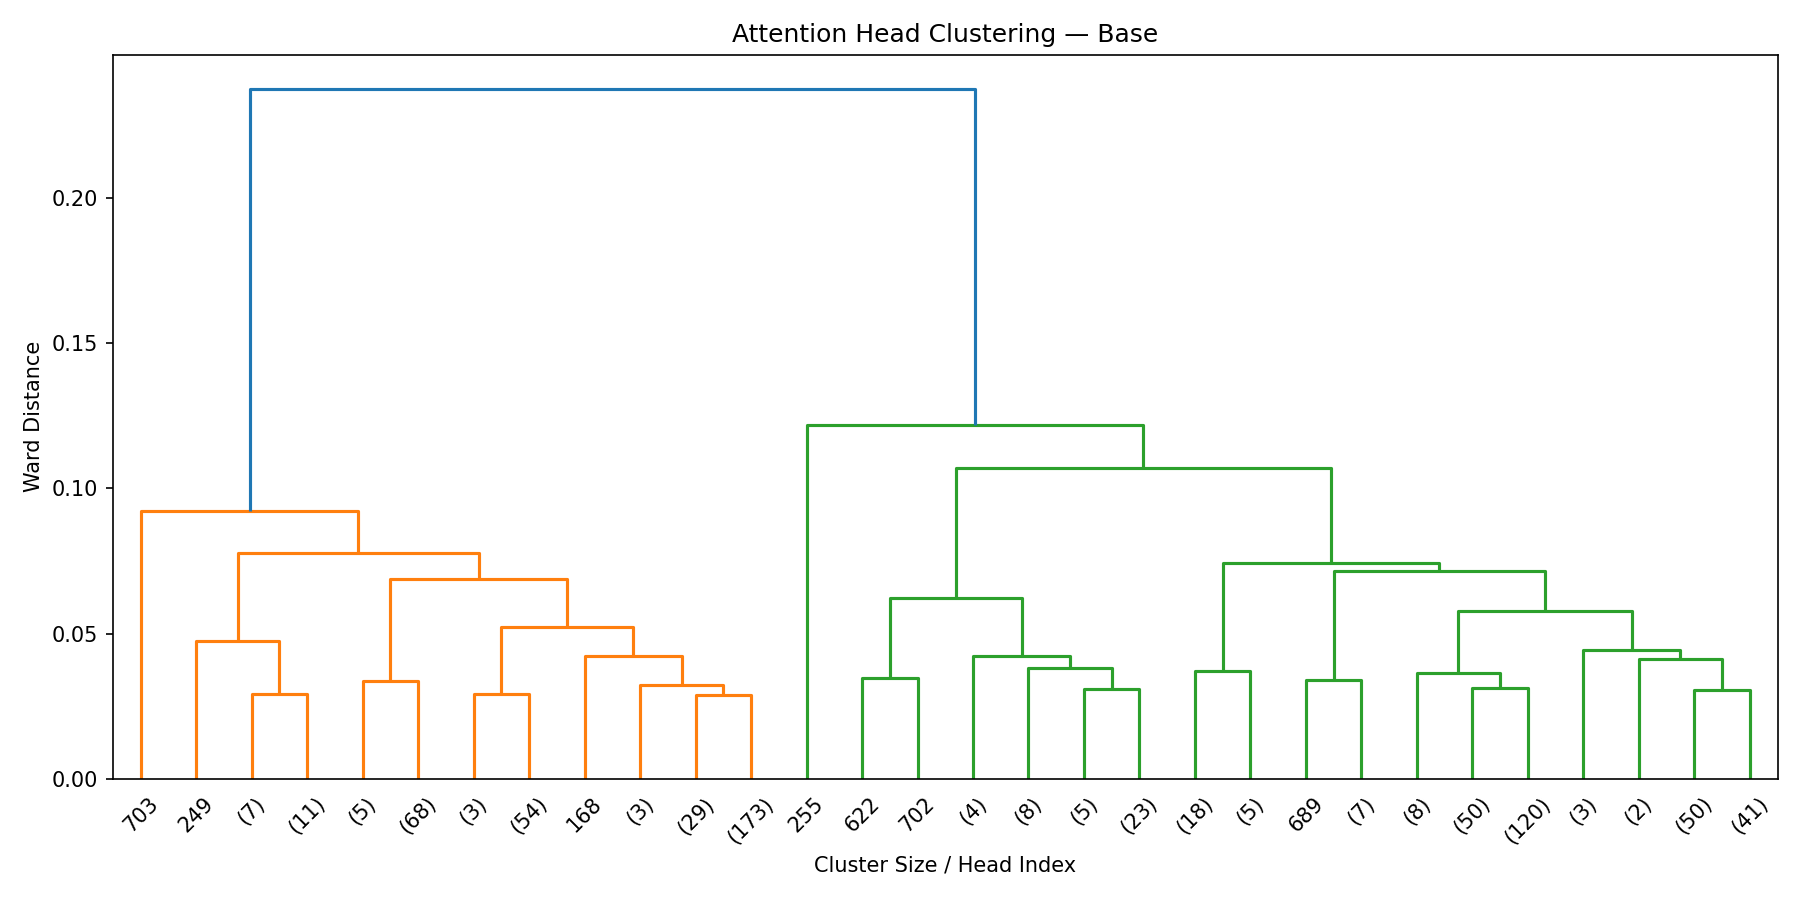
\includegraphics[width=0.485\linewidth]{../results/task3/head_clustering_Base.png}
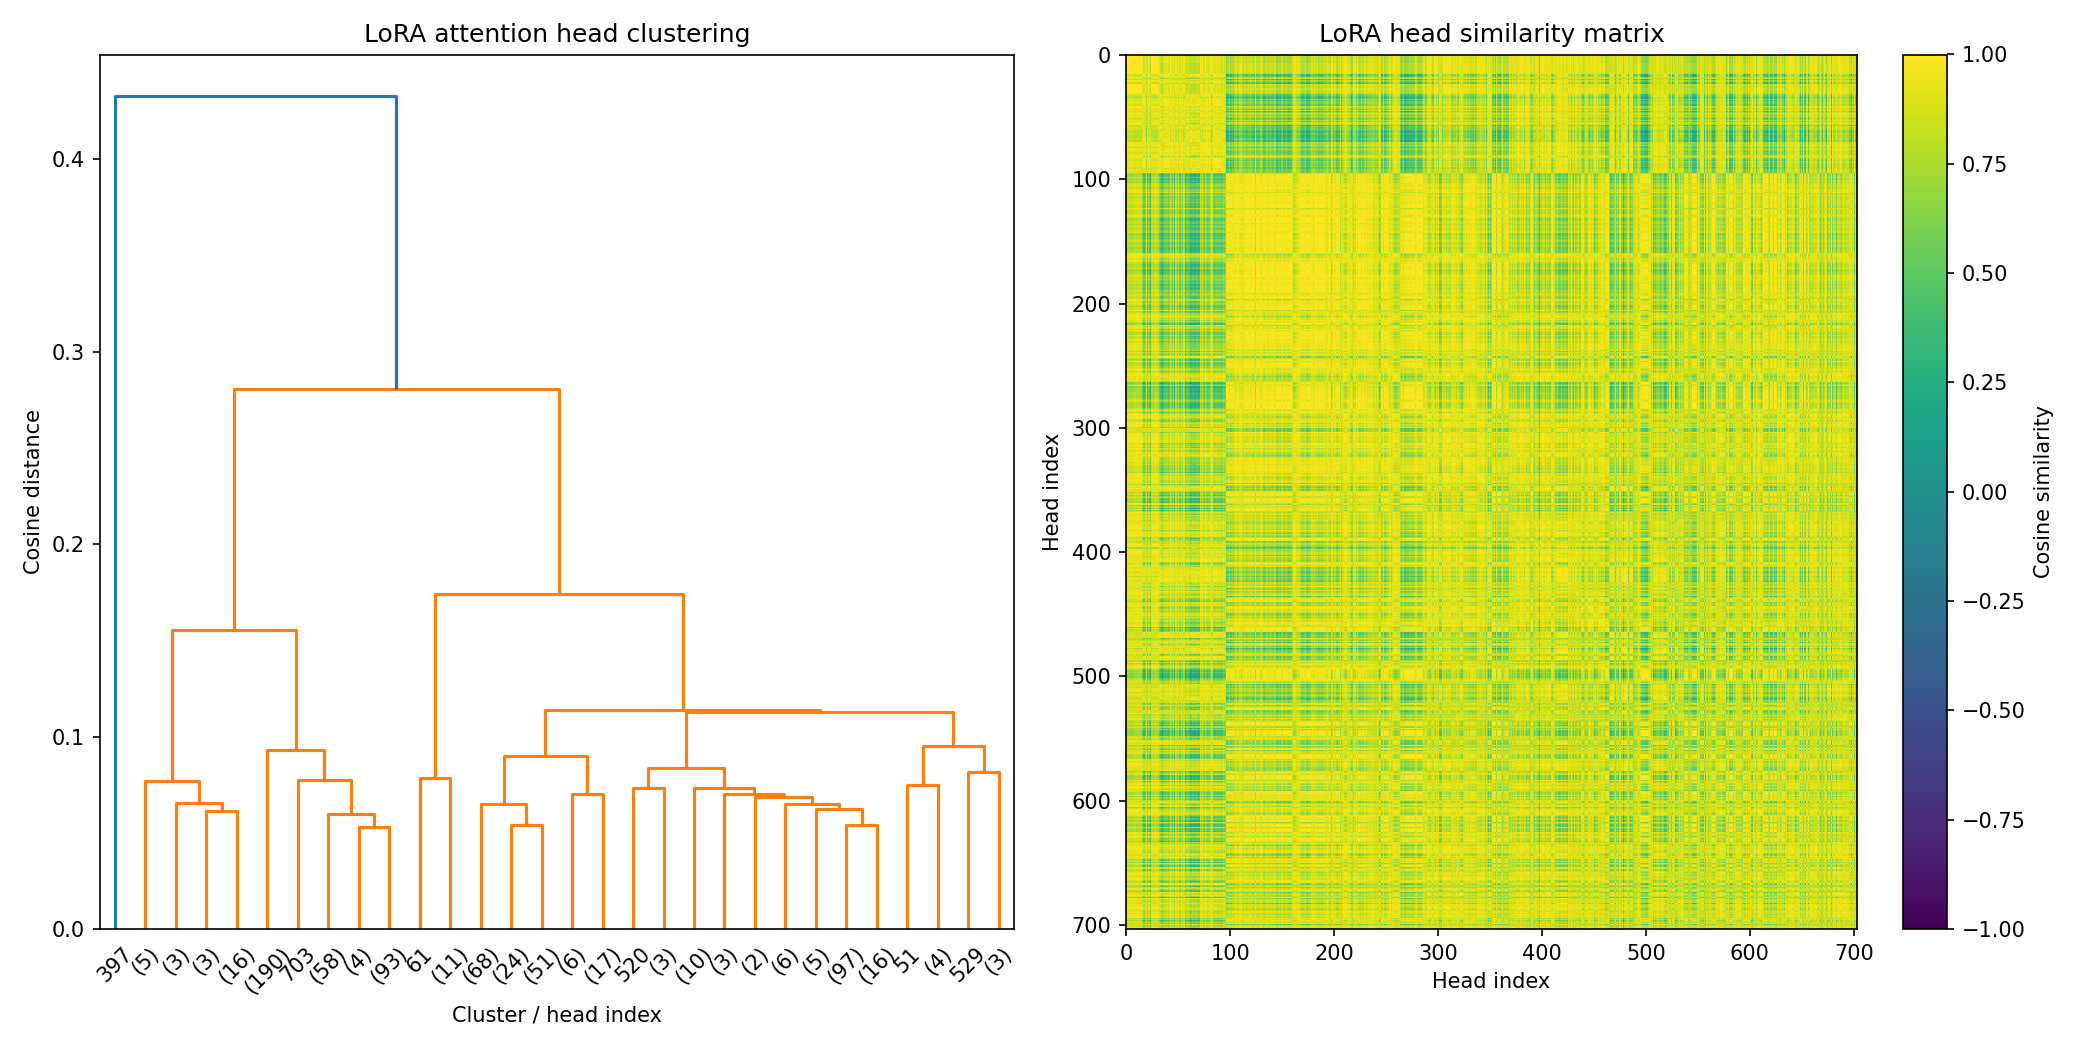
\includegraphics[width=0.485\linewidth]{../results/task3/head_clustering_LoRA.png}
\caption{Attention head clustering dendrogram topologies mapping base unsteered (left) vs Alpaca LoRA-tuned (right).}
\end{figure}

\begin{figure}[H]
\vspace{0.3cm}
\centering
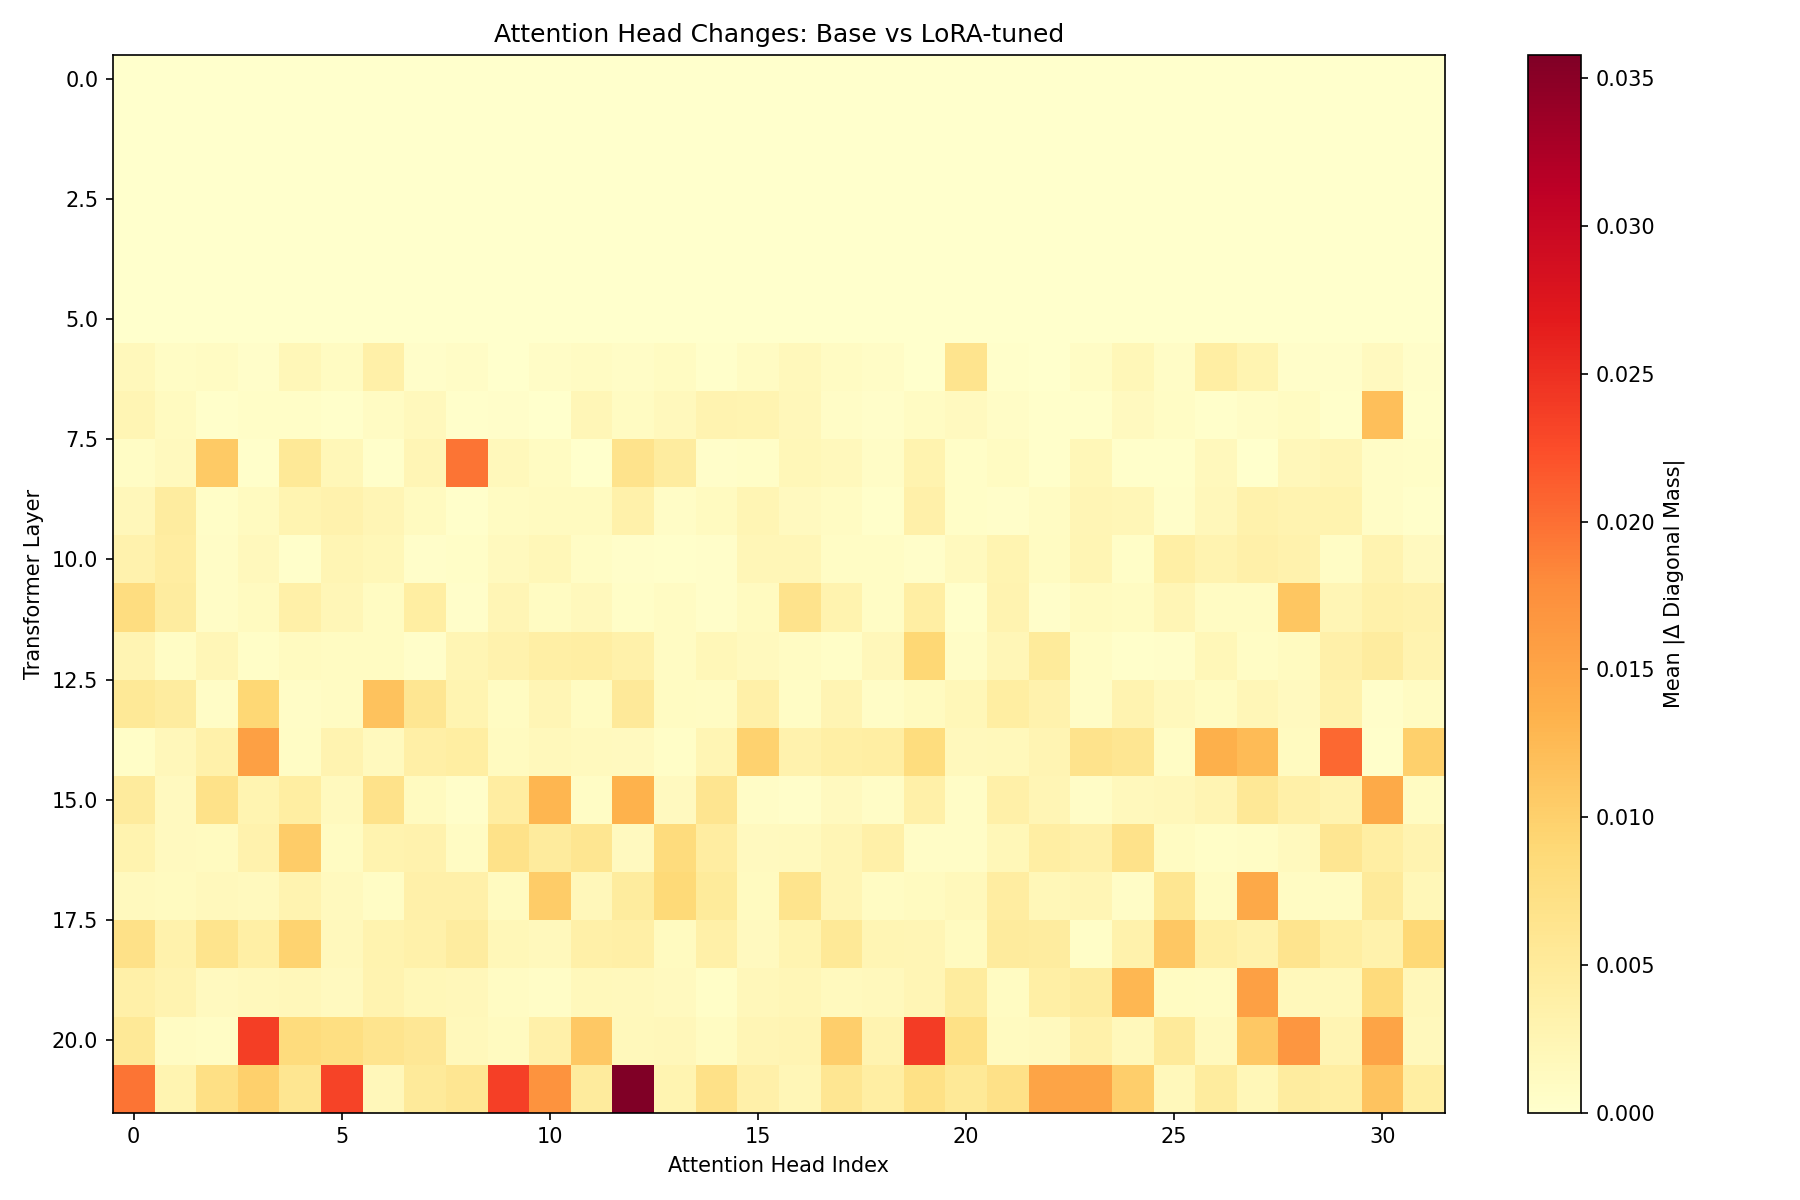
\includegraphics[width=0.49\linewidth]{../results/task3/base_vs_lora_attention_diff.png}
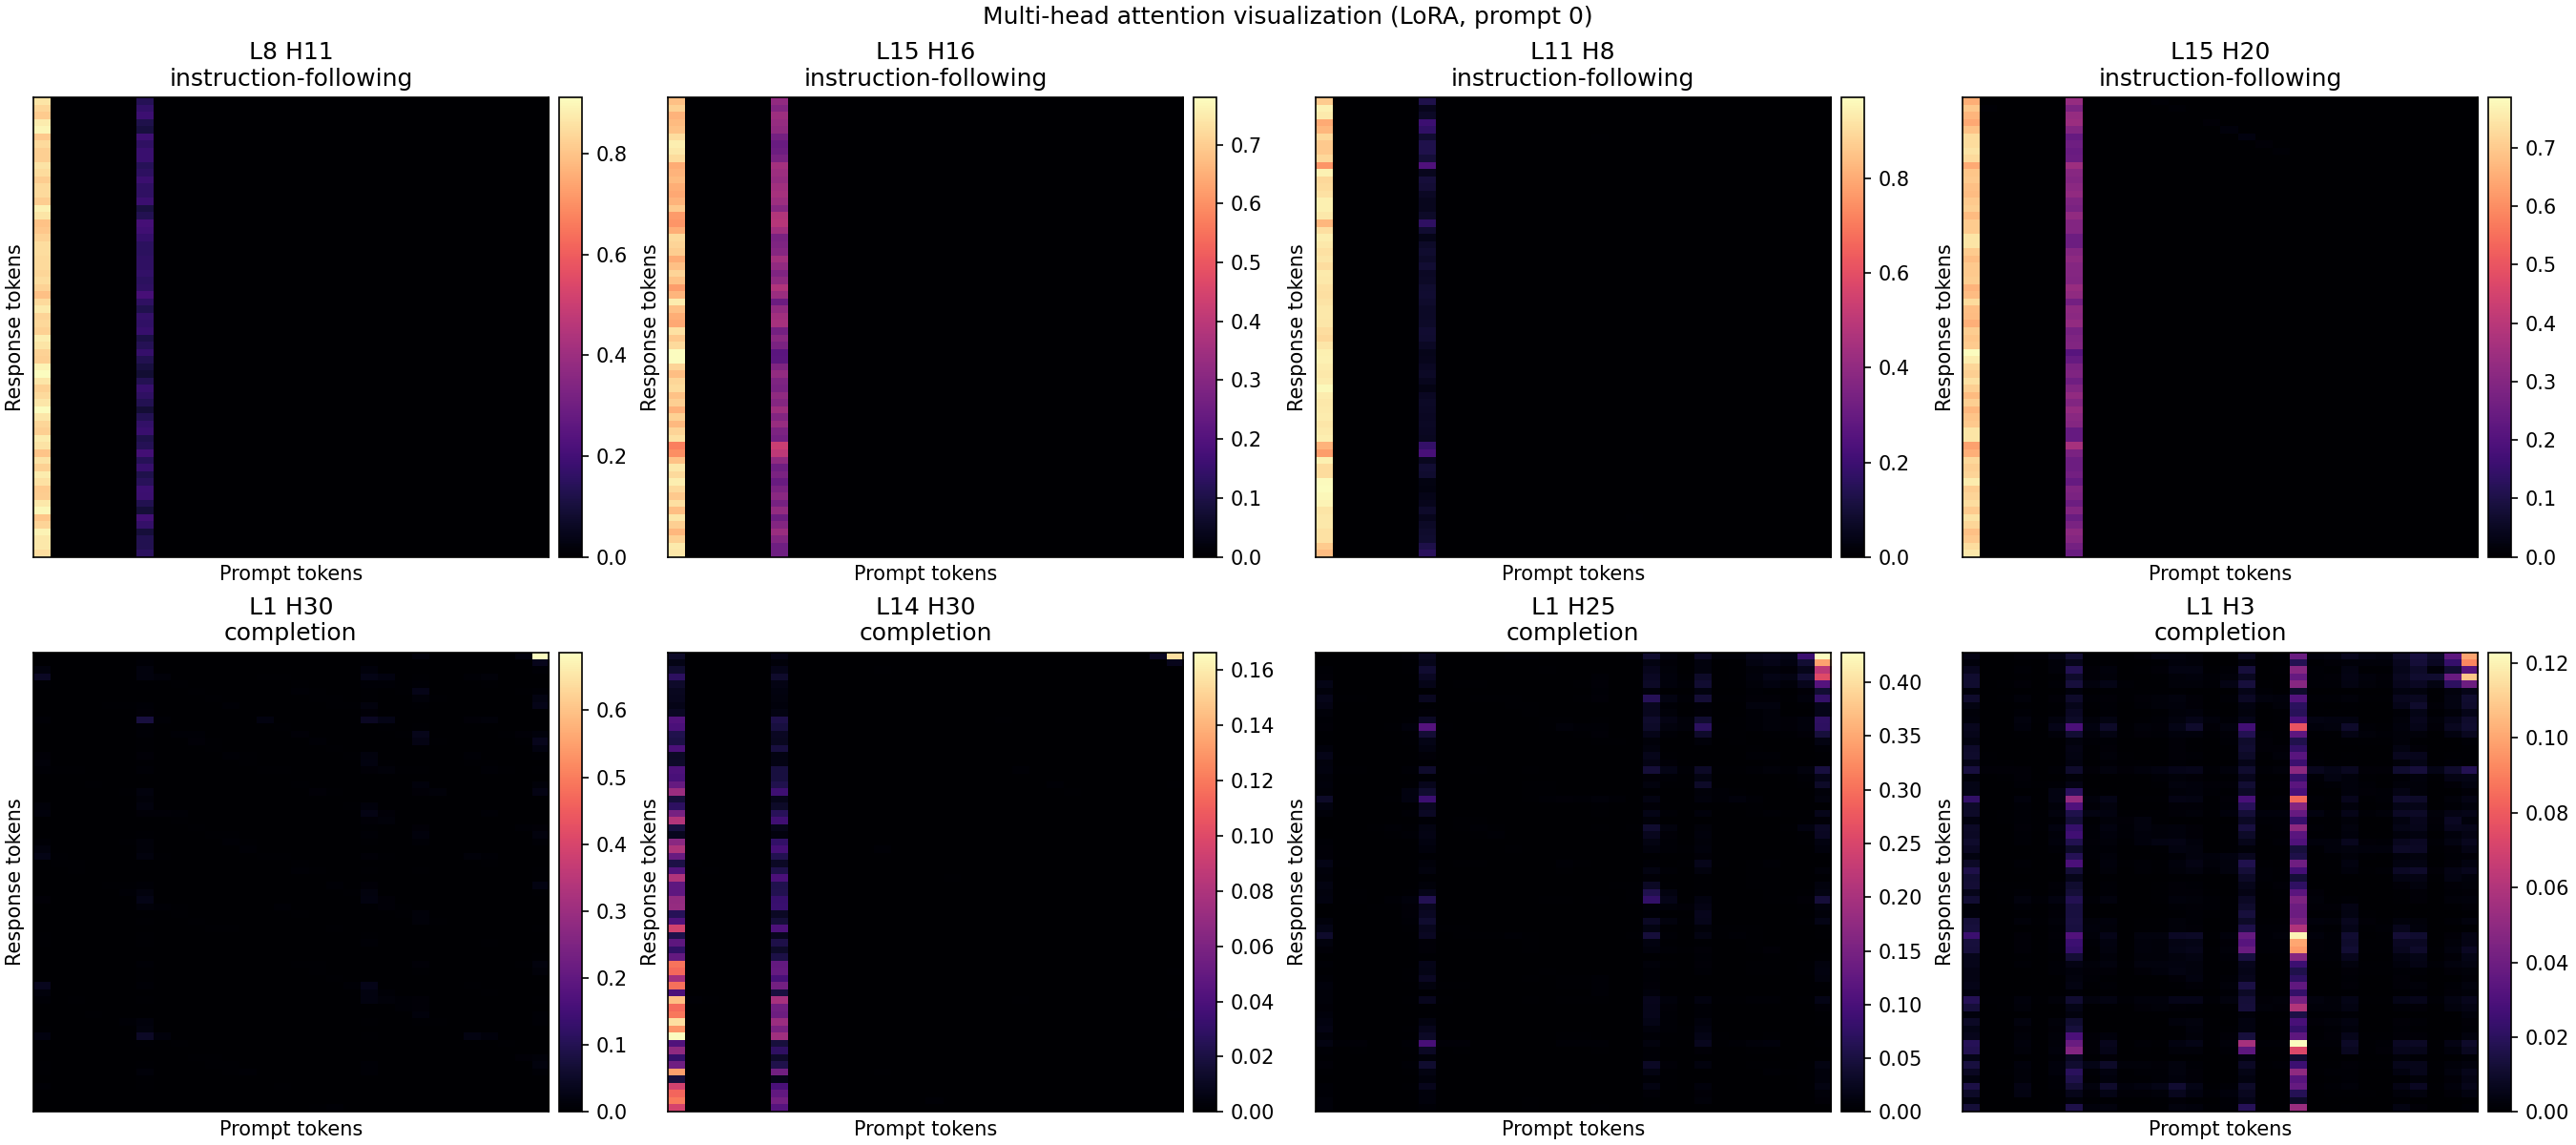
\includegraphics[width=0.49\linewidth]{../results/task3/multi_head_visualization.png}
\caption{\textbf{Left:} Scatter highlighting broad net-completion shift orientation. \textbf{Right:} Multi-head attention instruction vs. completion contrast graph mapping specific prompt tokens.}
\end{figure}

\end{document}
